%% Compiler: XeLaTeX

\documentclass[tikz,border=0pt]{standalone}%
\usepackage{tikz-cd}
\usetikzlibrary{arrows}

\begin{document}

%---------------------------ART-------------------------------------------------------------------------------------------%
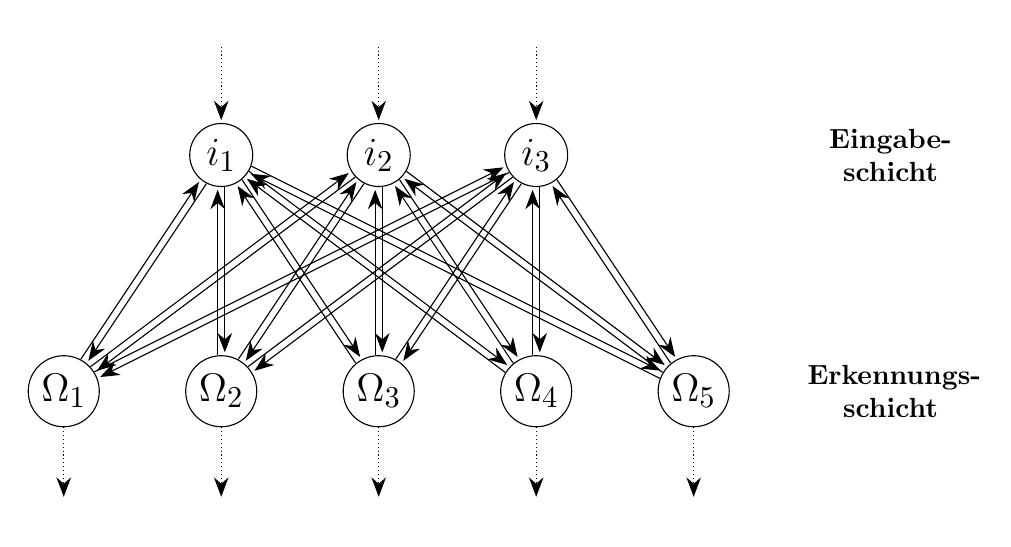
\begin{tikzpicture}[>=stealth', node distance=\layersep cm, shorten >=1pt]

        \def\layersep{3}            % vertikal distance between the layers
        \def\neuronsep{2}           % Horizontal distance between neurons
        \def\dlsize{2.5}            % distance between node and layer lable
        \def\inout{\layersep*.5}    % Size of in- and output-arrow
        \def\siz{.8}                % neuronsize
        \def\y{3}                   % Start of the most upper layer
        \def\ni{3}                  % Amount of input neurons
        \def\no{5}                  % Amount of output neurons
        \tikzstyle{neuron}=[circle,draw=black,minimum size=\siz cm,inner sep=2pt]
        \tikzstyle{annot} = [text width=6em, text centered]
        \tikzset{fontscale/.style = {font={\fontsize{#1pt}{#1pt}\selectfont}}}
        \tikzset{
            shift left/.style ={commutative diagrams/shift left={#1}},
            shift right/.style={commutative diagrams/shift right={#1}}
        }
        
        % Draw the left input layer nodes
            \foreach \xn in {1,...,\ni}{
                \node[neuron,fontscale=15] (Il-\xn) at (\xn*\neuronsep-\neuronsep,\y) {$i_{\xn}$};
                \node[above of=Il-\xn, node distance=\inout cm] (Inl-\xn) {};
                \draw [arrows={-Stealth[length=7pt]},densely dotted] (Inl-\xn) edge (Il-\xn);
            }
        % Draw the output layer node
            \foreach \xn in {1,...,\no}{
                \node[neuron] (Ol-\xn) at ({(\ni-1)*\neuronsep/2-\neuronsep/2*(\no-1)+(\xn-1)*\neuronsep},\y-\layersep) [fontscale=15] {$\Omega_{\xn}$};
                \node[node distance=\inout cm, below of=Ol-\xn] (Onl) {};
                \draw [->,arrows={-Stealth[length=7pt]},densely dotted] (Ol-\xn) edge (Onl);
        % Connect every node in the input layer with the output layer                
            \foreach \source in {1,...,\ni}{
                \draw [->,arrows={-Stealth[length=7pt]}, shift left=.3ex] (Il-\source) edge (Ol-\xn);
                \draw [->,arrows={-Stealth[length=7pt]}, shift left=.3ex] (Ol-\xn) edge (Il-\source);
                }}
                
        % Annotate the layers
                \node[annot,right of=Ol-\no, node distance=\dlsize cm] (ol) {\textbf{Erkennungs- schicht}};
                \node[annot,above of=ol] (il) {\textbf{Eingabe- schicht}};
                
        \end{tikzpicture}
\end{document}